\chapter{Navigating Textual Data: Dataset Insights and Preprocessing Techniques}
\label{chap:ch1}

\par
\section{Dataset Overview: Sourcing Mental Health Discussions from Subreddits}

\quad Our investigation relies on a carefully compiled dataset \cite{depressionDataset}, intentionally crafted to propel advancements in mental health classification research . Gathered through web scraping techniques from diverse Subreddits, this dataset encapsulates a broad range of discussions and viewpoints on mental health topics . The fundamental aim of creating this dataset was to facilitate a detailed examination of textual patterns indicative of depression's presence or absence in individuals, as inferred from their online conversations .

% \subsection{Collection Methodology}
The raw data was sourced by employing sophisticated web scraping techniques, targeting specific Subreddits known for their discussions on mental health issues. This approach ensured that the data collected was highly relevant to the research objectives, capturing a diverse range of experiences and expressions related to mental health.

% \subsection{Dataset Overview}
Comprising 7,650 unique entries, the dataset represents a rich tapestry of textual data. Each entry is meticulously annotated with an is\textunderscore depression label, distinguishing between texts that signify the presence of depression (labeled '1') and those that do not (labeled '0'). This labeling process was carried out with careful consideration to ensure accuracy and reliability in the classification \cite{depressionDataset}.

A noteworthy aspect of the dataset is its well-balanced nature, with 3,900 entries labeled as non-depression ('0') and 3,831 entries indicating depression ('1'). This balance is instrumental in avoiding bias in the predictive modeling process, ensuring that the resulting classification model is both fair and accurate. By maintaining an almost equal distribution between the two categories, the dataset provides a solid foundation for developing robust algorithms capable of detecting signs of depression in textual data.

Given the complexities and nuances of natural language, the raw data underwent a comprehensive cleaning process using multiple Natural Language Processing (NLP) techniques. This preprocessing phase was crucial for eliminating noise, such as irrelevant characters, web links, and non-English words, thereby refining the dataset for analysis. The cleaning process also involved normalizing the text to ensure consistency across the dataset, facilitating more effective data analysis and model training \cite{depressionDataset}.

In summary, the dataset presents a comprehensive and balanced collection of textual data aimed at enhancing our understanding and classification of mental health states, specifically depression, through the lens of online discourse. The careful curation, cleaning, and balancing of the data underscore the rigor and thoughtfulness applied in preparing this dataset for research purposes. This foundation sets the stage for applying advanced NLP techniques and machine learning models to unravel the complexities of mental health classification based on textual analysis.

\section{Leveraging LIWC-22 for In-depth Textual Analysis}

\quad In the realm of textual data analysis, especially within the context of psychological research, the tool we choose to process and interpret the data is as critical as the data itself. For this reason, our exploration of the dataset employs the latest version of a highly acclaimed text analysis software, LIWC-22 (Linguistic Inquiry and Word Count). This tool represents the culmination of decades of research and development in the field of computational linguistics and psychology, designed to uncover the intricate ways in which language reflects underlying psychological states.

LIWC-22 stands on the shoulders of giants, tracing its intellectual heritage back to early pioneers who first posited that the words we use in everyday communication are windows into our inner lives—revealing our thoughts, feelings, social relationships, and even our personalities. The tool is the product of a concerted effort to harness the power of computational methods to analyze language systematically, overcoming the complexities that early computer-based text analysis methods encountered \cite{boyd2022development}.

With LIWC-22, researchers have at their disposal a sophisticated software tool that not only builds upon the foundation laid by previous versions but also incorporates the latest advances in text analysis. Its expanded dictionary and enhanced software capabilities make it possible to analyze language samples with unprecedented depth and precision. Whether one is interested in exploring the nuances of emotional expression, social connectivity, cognitive processes, or any other psychological dimension manifest in text, LIWC-22 offers a robust and flexible platform for investigation.

In this section, we will explore the specific features of LIWC-22 that make it an invaluable tool for our research purposes, including its methodological underpinnings, its psychometric properties, and the ways in which it allows us to parse the subtle linguistic cues that signal varying psychological states. Through this exploration, readers will gain insight into the sophisticated interplay between language and psychology that LIWC-22 helps to elucidate, setting the stage for a deeper understanding of the dataset and the insights it holds.

\subsection{The Processing Capabilities of LIWC-22}

\quad The Linguistic Inquiry and Word Count (LIWC-22) tool stands as a cutting-edge solution for processing and analyzing textual data within the domain of psychosocial research. This sophisticated software, coupled with its comprehensive dictionary, bridges the gap between linguistic constructs and psychological theories, offering unparalleled insights into the psychosocial dimensions of language. Through a detailed overview of its primary and companion processing modules, we delve into how LIWC-22 serves as an indispensable tool for researchers aiming to uncover the psychological underpinnings of text \cite{boyd2022development}.

Upon analyzing texts, LIWC-22 quantitatively evaluates the language used against its expansive dictionary, calculating the percentage of words within each text that align with specific psychosocial categories. This process yields detailed metrics on the linguistic dimensions of the analyzed texts, which can be exported in various formats for further analysis.

Beyond its core functionality, LIWC-22 introduces several companion processing modules that enhance its analytical capabilities:

\begin{itemize}
\item Dictionary Workbench: Simplifying the creation of custom dictionaries, this module offers a user-friendly interface with built-in error checking. It facilitates the evaluation of custom dictionaries' psychometric properties, ensuring their effectiveness in research contexts \cite{boyd2022development}.

\item Word Frequencies and Word Clouds: These features assist in identifying the most common words within a dataset, providing visual word clouds for intuitive analysis of text samples \cite{boyd2022development}.

\item Topic Modeling with the Meaning Extraction Method: LIWC-22 incorporates the Meaning Extraction Method (MEM) for topic modeling, enabling researchers to uncover dominant themes and meanings within their datasets through factor analysis \cite{boyd2022development}.

\item Narrative Arc: This innovative module evaluates texts for narrative structures, offering insights into storytelling elements such as staging, plot progression, and cognitive tension \cite{boyd2022development}.

\item Language Style Matching (LSM): LSM analyzes the stylistic similarities between texts, offering metrics for comparing language use in various contexts, from individual communications to group dynamics \cite{boyd2022development}.

\item Contextualizer: Understanding the context of word use is vital. This module extracts words along with their surrounding text, allowing for a deeper examination of linguistic usage and implications \cite{boyd2022development}.

\item Case Studies: Tailored for in-depth analysis of individual texts, this module aggregates LIWC-22's capabilities to facilitate comprehensive study of specific documents or transcripts \cite{boyd2022development}.

\item Prepare Transcripts: Aiding in the preparation of conversation transcripts for analysis, this module streamlines the cleaning process, ensuring texts are optimized for LIWC analysis \cite{boyd2022development}.
\end{itemize}

Together, these modules position LIWC-22 as a versatile and powerful tool for linguistic and psychological research, offering novel ways to explore and interpret the complex interplay between language and psychosocial processes.

\subsection{The Evolution and Architecture of the LIWC-22 Dictionary}

\quad The LIWC-22 Dictionary is the linchpin of the Linguistic Inquiry and Word Count (LIWC) system, embodying the fusion of linguistic constructs with psychosocial theories through an extensive lexicon. This core component, comprising over 12,000 words, word stems, phrases, and select emoticons, is meticulously organized into categories and subcategories designed to capture a wide array of psychosocial constructs. This arrangement allows for a nuanced analysis of text, offering insights into the psychological state, social relationships, and cognitive processes of individuals based on their word usage.

Central to the LIWC-22 Dictionary's design is its hierarchical organization, where words are not only categorized but also interlinked across multiple dimensions. For instance, the word "cried" contributes to categories such as emotion, sadness, and past focus, illustrating the dictionary's complexity and depth. This structure enables LIWC-22 to provide a comprehensive analysis of text, reflecting various emotional and cognitive dimensions \cite{boyd2022development}.

The development of the LIWC-22 Dictionary represents a significant evolution from its predecessors, incorporating advances in computational linguistics and psychological research. The creation process involved multiple phases:
\begin{itemize}
\item Word Collection: Leveraging the foundation of the LIWC2015 dictionary, new words were generated for each category through a combination of expert input and comprehensive literature review \cite{boyd2022development}.
\item Judge Rating Phase: Words were qualitatively assessed by a panel of judges for their fit within each category, with disagreements resolved through in-depth analysis and consensus.
Base Rate Analyses: Utilizing the Meaning Extraction Helper (MEH) tool, the frequency of dictionary words in a diverse corpus was evaluated to ensure relevance and applicability across various text samples \cite{boyd2022development}.
\item Candidate Word List Generation: Through statistical analysis and expert review, candidate words were identified for potential inclusion in the dictionary, ensuring a broad and relevant lexicon \cite{boyd2022development}.
\item Psychometric Evaluation: Each category underwent rigorous testing for internal consistency, with adjustments made to optimize the dictionary's psychometric properties \cite{boyd2022development}.
\item Refinement Phase: The entire process was iteratively refined to address any oversights and enhance the dictionary's accuracy and reliability \cite{boyd2022development}.
\item Addition of Summary Variables: New summary variables were introduced to provide additional analytical dimensions, based on cutting-edge research \cite{boyd2022development}.
\end{itemize}

The LIWC-22 Dictionary has been significantly expanded to include not only traditional words but also numbers, punctuation, short phrases, and regular expressions. This expansion allows for the analysis of modern, informal communication styles found on social media and text messaging, incorporating "netspeak" and emoticons for a more comprehensive understanding of digital communication.

The dictionary's evolution reflects a balance between expert human judgment and sophisticated computational models, ensuring that LIWC-22 remains at the forefront of text analysis technology. With each iteration, LIWC has adapted to the changing landscape of language use, incorporating new categories and adjusting existing ones to better capture the psychological significance of language \cite{boyd2022development}.

In summary, the LIWC-22 Dictionary's development and structure are a testament to the interdisciplinary collaboration between linguistics and psychology. Its comprehensive and adaptable design makes it an invaluable tool for researchers and practitioners seeking to understand the deep psychosocial underpinnings of language use.

\subsection{The Psychometric Rigor of LIWC-22: Establishing Reliability and Validity}

\quad The development of the Linguistic Inquiry and Word Count (LIWC-22) tool has consistently prioritized the establishment of a scientifically robust system, focusing on both reliability and validity. This commitment has guided each iteration of LIWC, with the aim of adapting to the dynamic nature of language use and leveraging the expanding horizons of text-based data science. LIWC-22 represents the culmination of these efforts, integrating modernized dictionaries with cutting-edge data analytics to offer a highly validated tool for text analysis.

At the heart of LIWC-22's psychometric establishment is the "Test Kitchen" corpus [Figure \ref{FigKitchenCorpus}], a meticulously curated collection of English language samples drawn from a wide spectrum of sources. This corpus serves dual purposes: it is instrumental in the selection of words for the LIWC-22 dictionary and plays a crucial role in assessing the dictionary's reliability and validity. The breadth and diversity of the Test Kitchen corpus [Figure \ref{FigKitchenCorpus}] ensure that LIWC-22's analyses are grounded in a realistic representation of language use across various contexts \cite{boyd2022development}.

To capture the multifaceted nature of language, the Test Kitchen corpus [Figure \ref{FigKitchenCorpus}] was assembled from 15 distinct English language data sets, encompassing a wide range of communication forms, from blogs and emails to social media posts and movie dialogues. This comprehensive corpus consists of 15,000 texts, with each text sample reflecting the unique linguistic style of its author(s). The selection process for these samples was designed to include a diverse representation of texts, ensuring a broad coverage of language use in daily life.

The construction of this corpus involved selecting 1,000 text samples from each of the 15 sources, with each text containing at least 100 words. For longer texts, a specific algorithm was employed to extract a continuous segment of 10,000 words, ensuring a manageable and consistent analysis size. In total, the Test Kitchen corpus [Figure \ref{FigKitchenCorpus}] encompasses over 31 million words, providing a robust foundation for the validation and refinement of the LIWC-22 dictionary \cite{boyd2022development}.

Given the sensitivity and proprietary nature of some of the data sources, the Test Kitchen corpus, while invaluable for the development and testing of LIWC-22, cannot be made publicly available. This restriction underscores the careful consideration given to privacy and ethical research practices in the compilation and use of the corpus. Nevertheless, the corpus's diverse and extensive dataset has been crucial in fine-tuning LIWC-22's dictionaries to reflect genuine language usage patterns.

The meticulous construction of the Test Kitchen corpus and its application in developing LIWC-22 illustrate the comprehensive approach taken to ensure the tool's psychometric integrity. By grounding the dictionary in a wide-ranging and representative sample of English language use, LIWC-22 stands as a testament to the evolving field of text analysis, offering researchers a reliable and valid instrument for exploring the depths of linguistic and psychosocial phenomena \cite{boyd2022development}.

\begin{figure}[htbp]
	\centering
		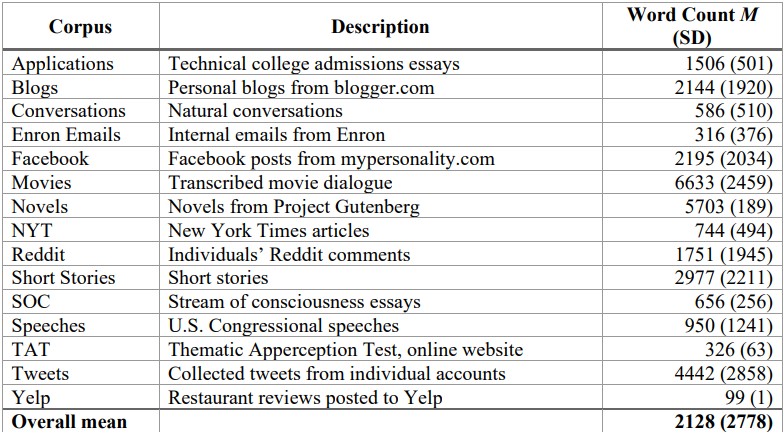
\includegraphics[scale=0.65]{./figures/test-kitchen-corpus.png}
	\caption{The test Kitchen Corpus of 31 Million Words \cite{boyd2022development}}
	\label{FigKitchenCorpus}
\end{figure}

\subsection{Challenges and Methodologies in Assessing LIWC-22's Psychometrics}

\quad The process of quantifying the reliability and validity of text analysis tools like LIWC-22 presents unique challenges, diverging significantly from the conventional approaches used in psychological assessments. The inherent differences between verbal behavior and structured questionnaire responses necessitate a nuanced approach to evaluating the psychometric properties of LIWC categories.

Unlike self-report questionnaires that gauge a construct like anger through multiple, similar questions to ensure internal consistency, natural language does not conform to such repetitive patterns. In real-world communication—be it a social media post, an essay, or a conversation—individuals express a thought and then naturally progress to the next, without the redundant expression of the same idea. This characteristic of verbal expression implies that the psychometric standards applied to language-based analyses must be recalibrated to account for the unique dynamics of verbal behavior \cite{boyd2022development}.

The evaluation of LIWC-22's reliability involves an innovative adaptation to the language's non-repetitive nature. Taking the LIWC-22 Anger scale as an instance, the scale encompasses 181 words and phrases associated with anger. Theoretically, the usage of one anger-related word in a text should correlate with the usage of other anger-related words within the same text. By analyzing how each of these words is employed across a selection of texts and calculating the intercorrelations among these word usages, LIWC-22's approach to determining internal consistency emerges\cite{boyd2022development}.

Validating the numerous LIWC dimensions poses a significant and complex challenge. By their nature, LIWC's content categories appear to be directly relevant or face valid. Yet, the deeper question lies in determining the extent to which both personal and social psychological processes are mirrored in the use of language. For instance, the implications of using words related to "affiliation" at a high frequency raise questions about the user's social connections and needs. Are individuals using these words seeking more social interaction, or do they reflect a person's existing strong social ties? Additionally, it is important to consider whether the frequency of such language usage offers insights into or predictions about someone's social relationships and needs.

To compute these metrics, LIWC-22 employs two statistical methods: the Cronbach’s alpha (\textalpha) for continuous data, based on the percentage of total words, and the Kuder–Richardson Formula 20 (KR-20) for binary data \cite{kuder1937theory}, indicating the presence or absence of words. These methods yield insights into the internal consistency of the LIWC-22 categories, adapting traditional psychometric calculations to the context of language analysis \cite{boyd2022development}.

The application of Cronbach’s alpha in the context of LIWC-22 encounters a significant hurdle due to the variable base rates of word usage within language categories. This variability can lead to underestimations of reliability when using traditional methods. Conversely, the Kuder–Richardson Formula 20 offers a more accurate reflection of a category's internal consistency by accommodating the binary nature of word presence, thus providing a "truer" approximation of reliability in language analysis.

The volume of research at the intersection of text analysis and psychosocial processes is vast, with over 2,400 studies cited in 2021 alone that utilized LIWC for text analysis. Findings from these studies, including those from the developers' own laboratories, reveal correlations between the affect or emotion categories detected by LIWC in texts and the authors' self-reported feelings. These correlations, although modest, underscore the tool's capability to capture psychological dynamics to a certain extent. Higher correlations are observed when comparing judges' ratings of writing samples with LIWC scores, suggesting a somewhat consistent external validation of LIWC's analytical output\cite{boyd2022development}.

The methodologies adopted for assessing the reliability and validity of LIWC-22 underscore the tool's sophisticated approach to text analysis. By carefully navigating the intricacies of natural language and employing tailored statistical methods, LIWC-22 achieves a nuanced and psychometrically sound analysis of verbal behavior. This approach not only highlights the challenges inherent in language-based psychometrics but also showcases LIWC-22's commitment to providing reliable and valid insights into the psychological underpinnings of text.

\section{Tokenization for LIWC-22 Compatibility}

\quad We shall delve into the tokenization method utilized in our study, designed to preprocess text data to ensure it aligns with the requirements of the Linguistic Inquiry and Word Count (LIWC-22) tool \cite{boyd2022development}. LIWC requires input texts to be broken down into tokens, a process that can significantly influence the accuracy and reliability of the linguistic analysis. Our chosen methodology leverages the strengths of BERT's tokenization system, as described in the referenced study \cite{bertTokenizerEnglish}.

BERT, or Bidirectional Encoder Representations from Transformers, introduces a sophisticated approach to tokenization that we adapted for our needs. BERT’s tokenization algorithm is based on WordPiece \cite{wu2016google}, handling the input text by initially breaking it down into tokens, which are then further divided into sub-tokens. This mechanism allows for a fine-grained understanding of language, capturing nuances by analyzing tokens in the context of their surrounding text.

The BERT model is pre-trained on a vast corpus of text, allowing it to understand a wide range of linguistic nuances. Its bidirectional nature means that each token is influenced by the tokens that come before and after it, providing a rich context for each word. This context is crucial for accurate linguistic analysis, as the meaning of a word can change significantly depending on its context \cite{bertTokenizerEnglish}. For example, in the sentence “I read that book,” the tokenization process needs to understand whether "read" is in the past or present tense, which has implications for the psychological constructs that LIWC-22 might extract.

By using BERT's tokenization, we ensured that our model could handle the complexity of the text data typically found on platforms like Reddit. This is particularly important for detecting signs of depression, where context can change the sentiment or meaning of a word. Furthermore, the sub-token approach allowed us to maintain the granularity needed for LIWC-22 \cite{boyd2022development}, which often relies on the detection of specific words and categories relevant to psychological states.









